\label{sec:risk-assessment}
The following tables identify various risks and hazards associated with the use of our aircraft, following a standard University of Melbourne Risk Assessment template, shown in Figure \ref{fig:risk-matrix}.\\

Each row of the risk assessment tables contains the following information: the potential hazard, the likelihood of that hazard occurring during the mission, a ``rating'' of the consequence of that hazard, and an assessment of the overall risk for that hazard. Management and mitigation of these risks will be discussed in Section \ref{sec:risk-management}.

\begin{figure}[H]
	
	\begin{subfigure}{\linewidth}
		\centerline{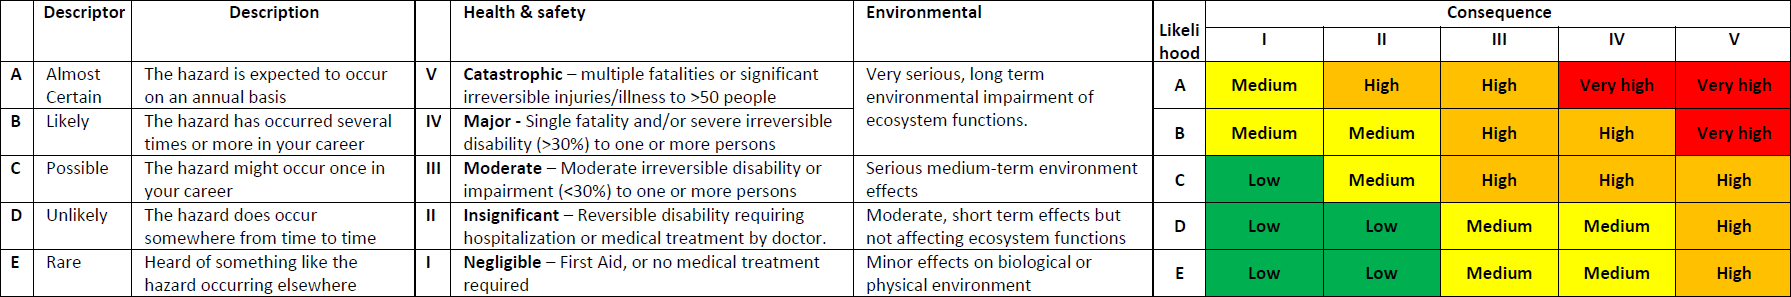
\includegraphics[width=550pt]{../Images/risk-matrix}}
	\end{subfigure}\\[2ex]
	
	\begin{subfigure}{\linewidth}
		\centerline{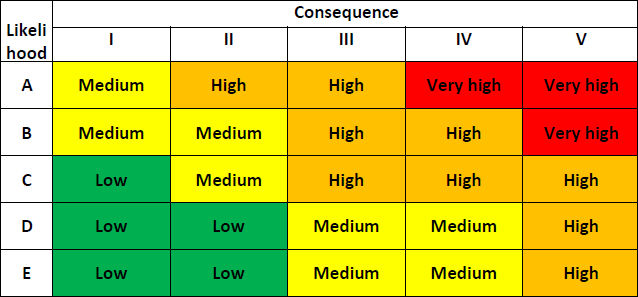
\includegraphics[width=300pt]{../Images/risk-matrix-2}}
	\end{subfigure}
	
	\caption{Risk Management Matrix}
	\label{fig:risk-matrix}
\end{figure}

\begin{table}[!h]
	\label{tab:risks-electrical}
	\centering
	\begin{tabularx}{\textwidth}{|Y|c|c|c|}
		\hline
		\textbf{Risk} & \textbf{Likelihood} & \textbf{Consequence} & \textbf{Risk Rating}\\
		\hline
		Electrocution & Possible & Insignificant & Medium\\
		\hline
		Impact to batteries & Possible & Insignificant & Medium\\
		\hline
		Loss of motor power & Possible & Insignificant & Medium\\
		\hline
	\end{tabularx} 
	\caption{Risk Assessment - Electrical Hazards}
\end{table}

\begin{table}[!h]
	\label{tab:risks-preflight}
	\centering
	\begin{tabularx}{\textwidth}{|Y|c|c|c|}
		\hline
		\textbf{Risk} & \textbf{Likelihood} & \textbf{Consequence} & \textbf{Risk Rating}\\
		\hline
		 & & & \\
		\hline
	\end{tabularx} 
	\caption{Risk Assessment - Pre-flight Hazards}
\end{table}

\begin{table}[!h]
	\label{tab:risks-autonomy}
	\centering
	\begin{tabularx}{\textwidth}{|Y|c|c|c|}
		\hline
		\textbf{Risk} & \textbf{Likelihood} & \textbf{Consequence} & \textbf{Risk Rating}\\
		\hline
		& & & \\
		\hline
	\end{tabularx} 
	\caption{Risk Assessment - Autonomous Takeoff and Landing}
\end{table}

\begin{table}[!h]
	\label{tab:risks-inflight}
	\centering
	\begin{tabularx}{\textwidth}{|Y|c|c|c|}
		\hline
		\textbf{Risk} & \textbf{Likelihood} & \textbf{Consequence} & \textbf{Risk Rating}\\
		\hline
		Loss of aircraft control & Possible & Insignificant & Medium \\
		(Autopilot failure or lock-up) & & & \\
		\hline
		Loss of aircraft control  & Likely & Insignificant & Medium \\
		(Propeller or power loss) & & & \\
		\hline
		Loss of GPS link only to GCS & Likely & Insignificant & Medium \\
		\hline
		Loss of telemetry/radio link only to GPS & Likely & Insignificant & Medium \\
		\hline
		Loss of both telemetry and GPS to GCS & Possible & Insignificant & Medium \\
		\hline
		GCS failure & Possible & Insignificant & Medium \\
		(aircraft loses communication with GCS) & & & \\
		\hline
		Geofence breach & Likely & Insignificant & Medium \\
		\hline
	\end{tabularx} 
	\caption{Risk Assessment - In-flight Hazards}
\end{table}

\begin{table}[!h]
	\label{tab:risks-other}
	\centering
	\begin{tabularx}{\textwidth}{|Y|c|c|c|}
		\hline
		\textbf{Risk} & \textbf{Likelihood} & \textbf{Consequence} & \textbf{Risk Rating}\\
		\hline
		Aircraft not operational or not controllable & Possible & Insignificant & Medium \\
		\hline
		Risk of injury to persons near aircraft & Possible & Insignificant & Medium \\
		\hline
	\end{tabularx} 
	\caption{Risk Assessment - Other Hazards}
\end{table}